\documentclass[a4paper]{article}

\usepackage[francais]{babel}
\usepackage{amsmath}
\usepackage{graphicx}
\usepackage{fontspec}
\usepackage{listings}
\usepackage{moreverb}
\usepackage{color}
\usepackage{hyperref}
\usepackage[colorinlistoftodos]{todonotes}
\usepackage[labelformat=empty]{caption}
\usepackage[textwidth=17cm]{geometry}

%\setlength{\textwidth}{420 pt} 

\lstset{language=Python,
frame=lines,
basicstyle=\fontsize{9}{11}\selectfont\ttfamily,
numbers=left,
breaklines=true,
showstringspaces=false,
tabsize=3}

\title{Systèmes multi-agents : la bille, le poisson et l'avatar}

\author{Matthieu CARON - Alexandre MOEVI}

\date{\today}

\begin{document}
\maketitle

\section{Architecture et utilisation}

\subsection{UMLUL}
\url{http://modeling-languages.com/uml-tools/#python}

\subsection{Usage}

\$PYTHONPATH, python3, modifier les paramètres dans MainXXX.py, etc.
\section{Simulations}

\subsection{Tube à particules}

La première simulation, le paquetage \textit{particules} consiste à reproduire le comportement de billes (ou particules) dans un espace. Cet espace peut torique ou non ; s'il ne l'est pas, les particules rebondissent contre les murs. Les particules rebondissent également en collision.

\medskip
La classe Bille

\subsection{Poissons et requins dans le golfe (du Bénin)}
What
 
\begin{figure}[!h]
\centering
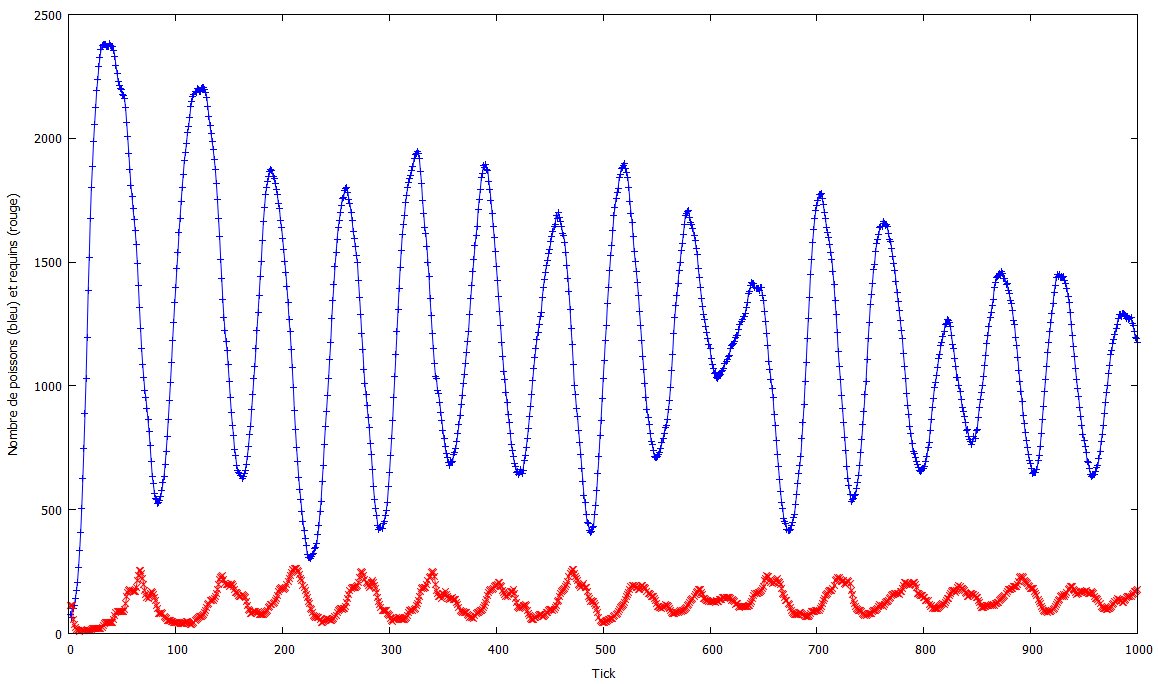
\includegraphics[height=10cm]{1000tours.png}
\caption{Courbes de population.}
\end{figure}

WHY
\subsection{Pac-Man}

\end{document}